\subsection{Support fit and future error}
We record the original target-update trajectory for the deeper and matched GRUs across all cities, budgets and seeds. Additional controls reduce the learning rate tenfold, freeze all but the output head, or penalize squared parameter movement from the pretrained weights ($\lambda=0.01$ or $0.1$)~\cite{l2sp}. The controls use the original support batches and optimizer for each backbone. The 216 zero-step and original-endpoint replay checks agree with archived forecasts within $1.2\times10^{-5}$ AQI points.

The deep pooled GRU starts at 26.669 macro MAE in 2025, averaged across the budgets and horizons. After its original 100 Adam updates at 0.0003, MAE rises by 10.960 points in 2025 (14-day block interval $[8.813,12.991]$) and by 8.579 in 2024. The 2025 increases at 30, 90 and 180 labels are 21.381, 8.250 and 3.248; larger budgets also extend the support window. Mean residual MSE on the fitting labels falls by 0.0672 in scaled units. The support MSE falls and 2025 MAE rises together in 149/162 city--budget--seed--horizon cases. MAE also rises by 9.356 on the fixed donor refit panel, which measures retention of donor training performance.

For initial error $e=\widehat y_0-y$ and adaptation correction $d=\widehat y_1-\widehat y_0$, the change in squared error is $2ed+d^2$. In 2025 the mean cross term is $-132.0$ AQI$^2$, indicating that the correction has a favorable mean projection against the initial errors. Its mean squared size is $1,224.7$ AQI$^2$, which dominates and raises MSE by $1,092.7$ AQI$^2$. This shows that large changes are sufficient to account for the net squared-error increase even when their aggregate direction is favorable.

At the same 100 updates, the 2025 MAE rise shrinks to 0.606 with the lower learning rate, 1.853 with head-only adaptation, and 7.021 or 3.371 with the weaker or stronger weight anchor (Fig.~\ref{fig:adaptationdiagnostics}). Each control limits parameter movement. The matched GRU's original three SGD updates at 0.01 change 2025 MAE by only $+0.008$ (14-day block interval $[-0.089,0.114]$), while thirty updates raise it by 0.724. The interventions trace much of the deep-GRU loss to the size and freedom of the target update. The experiment leaves the environmental source of the support-to-query difference open.

\begin{figure}[t]
\centering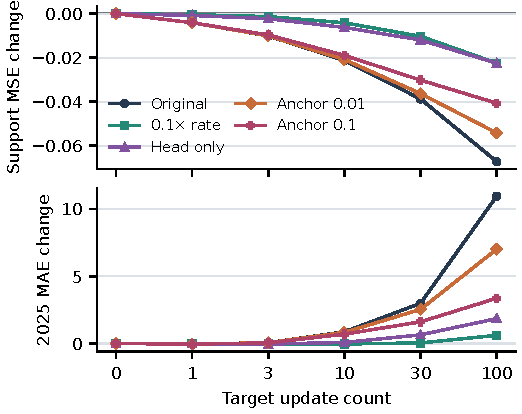
\includegraphics[width=\columnwidth]{adaptation_diagnostics.pdf}
\caption{Deep-GRU changes from the pooled checkpoint. The support panel shows scaled residual MSE and the 2025 panel shows AQI MAE. Both average across cities, budgets, horizons and seeds. Checkpoint positions are equally spaced on the axis.}
\label{fig:adaptationdiagnostics}
\end{figure}
